\chapter{INTRODUCTION\label{chapter:introduction}}
The nature of scientific models is a deep philosophical topic \citep{giere2010explaining}, \citep{morrison2009models}, \citep{frigg2006models}.
Scientific models play an integral role in making predictions about as well as explaining how aspects of the physical world behave.
For the purposes of this thesis, we will consider a very abstracted view of scientific models as assertions about a collection of variables that refer to aspects of the world, along with a set of functional relations between variables that stipulate how the state of one variable is a function of zero or more other variables.
This form of scientific model can be depicted as a graph, such as the model shown in Fig~\ref{fig:example_sci_model}.
As shown in the figure, scientific models can be used to study real-world systems by providing sets of inputs values to the model and observing the model outputs.

\begin{figure}[!htbp]
  \label{fig:example_sci_model}
  \centering
  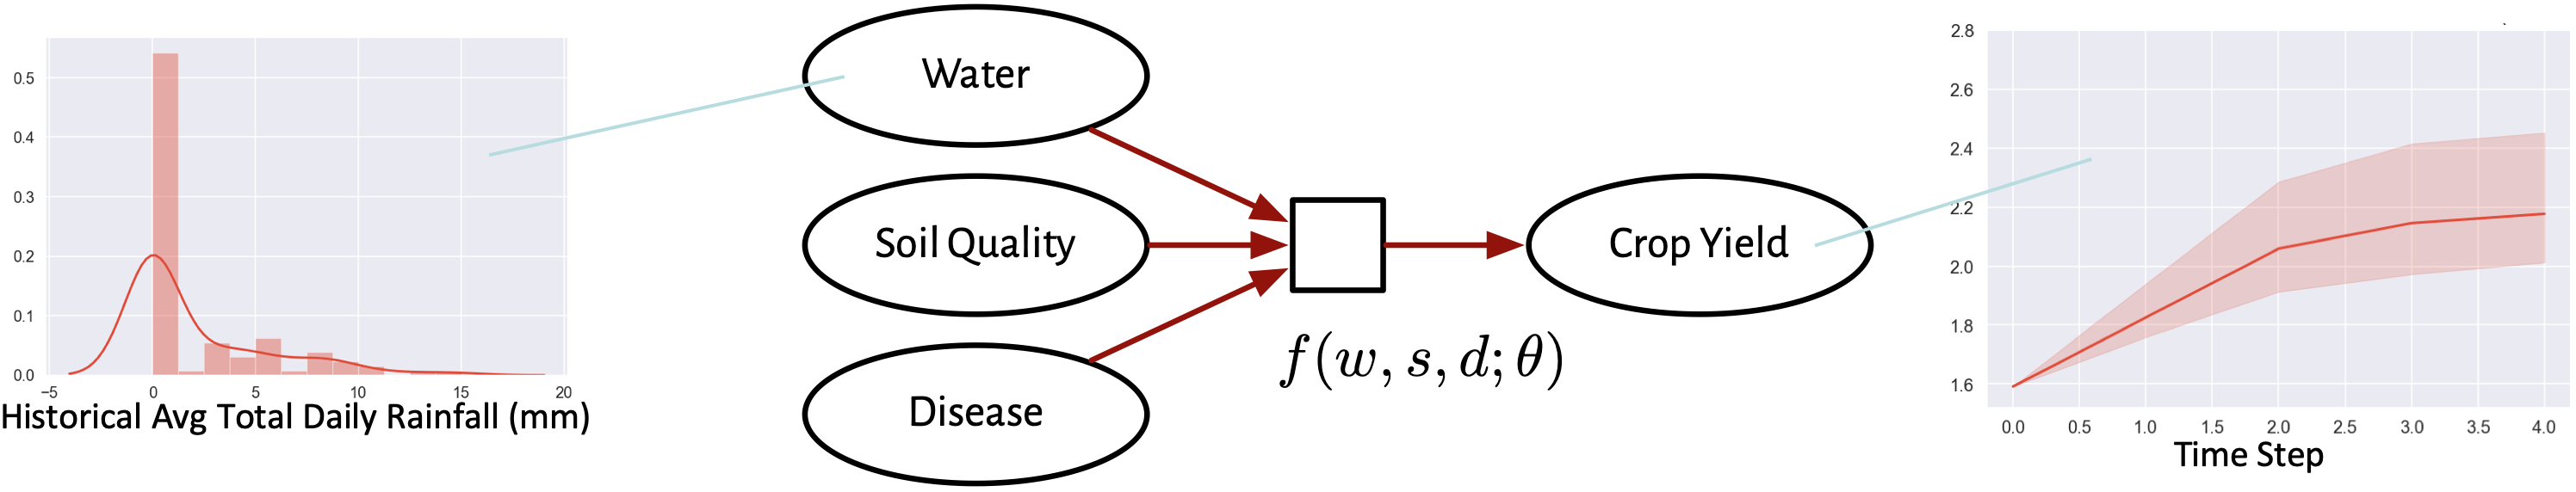
\includegraphics[width=\textwidth]{example_scientific_model}
  \caption[An Example of a Scientific Model]{An illustration of a scientific model that shows how a distribution over a model input can be used to make predictions about the models output.}
\end{figure}


Scientific models are explicit explanations of how observable phenomena influence one another as a system.
For the purposes of this thesis, a scientific model will be thought of as a collection of variables that form a system as well as a set of functional relations upon the variables.
Scientific models are particularly useful when they facilitate the ability to predict the output of a system, given observations of the systems inputs.
For many systems of observable phenomena that domain modelers are interested in studying multiple competing scientific models of the system exist.
An example of such a situation is shown in Figure~\ref{fig:simple_crop_CAG} which depicts two competing scientific models of a system of variables that seeks to describe how the yield of a particular crop is affected by changes in the amount of rain and soil water absorption rate over time (expressed in \emph{Day}s).

\begin{figure}[!htbp]
  \label{fig:simple_crop_CAG}
  \centering
  \tikz{ % Simple Crop Yield model example
    \tikzstyle{readable}=[rectangle, thick, rounded corners]
    \node[latent, readable] (crop_yield) {$Yield$} ; %
    \node[latent, readable, above=of crop_yield] (total_rain) {$Rain_{total}$} ; %
    \node[latent, readable, above=of total_rain] (rain) {$Rain$} ; %
    \node[obs, readable, above=of rain] (max_rain) {$Rain_{max}$} ; %
    \node[obs, readable, left=of max_rain] (absorption) {$Absorption$} ; %
    \node[obs, readable, right=of max_rain] (consistency) {$Consistency$} ; %
    \node[obs, readable, right=of rain] (day) {$Day$} ; %
    \edge {day, consistency, absorption, max_rain} {rain} ; %
    \edge {rain} {total_rain} ; %
    \path [->] (total_rain) edge  [loop right] (total_rain);
    \edge {total_rain} {crop_yield} ; %

    \plate {loop} {(rain)(day)(total_rain)} {$Day$} ;
  }
  \tikz{ % Different Crop Yield model example
    \tikzstyle{readable}=[rectangle, thick, rounded corners]
    \node[latent, readable] (crop_yield) {$Yield$} ; %
    \node[latent, readable, above=of crop_yield] (total_rain) {$Rain_{total}$} ; %
    \node[latent, readable, above=of total_rain] (rain) {$Rain$} ; %
    \node[obs, readable, above=of rain] (max_rain) {$Rain_{max}$} ; %
    \node[obs, readable, right=of max_rain] (absorption) {$Absorption$} ; %
    \node[obs, readable, left=of rain] (consistency) {$Consistency$} ; %
    \node[obs, readable, left=of total_rain] (sunlight) {$Sunlight$} ; %
    \node[obs, readable, right=of rain] (day) {$Day$} ; %
    \edge {day, absorption, max_rain} {rain} ; %
    \edge {rain, consistency} {total_rain} ; %
    \path [->] (total_rain) edge  [loop right] (total_rain);
    \edge {total_rain, sunlight} {crop_yield} ; %

    \plate {loop} {(rain)(day)(total_rain)} {$Day$} ;
  }
  \caption[Competing Models of Crop Yield]{Two competing scientific models depicting the affects of rain on the yield of a crop over a span of days given a set of input variables (shaded). We see that the two models share many of their inputs but that some inputs may not be shared and the wiring of the inputs to the output variable differs between the two models.}
\end{figure}

We can see that, while the two scientific models shown in Figure~\ref{fig:simple_crop_CAG} share many variables, some variables are not shared between the two models, and the wiring between these two models is not identical.
This presents a problem to domain modelers, which of these models is more suitable to use when studying the crop yield system?
This question is formalized as the model choice problem.
The model choice problem requires domain modelers to analyze the available competing models of their system of interest and then to select which model will best describes the system for their experimental data.
The process of analyzing the available scientific models of a system is formalized as the task of scientific model analysis.
Scientific model analysis involves the analytical study of scientific models to gain information about one or more scientific models that can be used as metrics of model fitness for a given experiment.
These metrics of model fitness are especially useful when they are comparative across models such that they can be used to differentiate competing models of the same phenomena.
This entails that the model choice problem can be solved by effectively conducting the task of model analysis.


\section{Motivation\label{sec:motivation}}
Performing the task of model analysis upon scientific models can be described as the following process:
\begin{enumerate}
  \item Find all competing scientific models for the system of interest
  \item Formally describe the scientific models as executable computational graphs
  \item Utilize mathematical methods of structural and functional analysis to gather comparative metrics that differentiate the scientific models performance
\end{enumerate}

domain modelers normally accomplish the first step of the process of model analysis by reading through the scientific literature to discover scientific models of the systems of phenomena they are interested in studying.
Fortunately, in recent years, the scientific models presented in the scientific literature are increasingly expressed as executable software.
This enables a host of opportunities, including the following:
\begin{itemize}
\item increased precision in predictions,
\item the possibility of better control over reproducibility of results,
\item better communication of model details through unambiguous code implementation, and
\item the potential to aggregate individual models from different domains into larger multi-domain models.
\end{itemize}
These advantages have been the driving force that has pushed the scientific community towards computational models as a method of communicating scientific  models in their research.
Now that these models-as-software are becoming the common currency of scientific discourse and methodology, completing the first task of the model analysis process largely solves the second task as well.
When scientific models are expressed in source code, not only do they benefit from all of the items outlined above, but the models are instantly executable as computation graphs.

However, having access to the source code implementation of scientific models is not sufficient to satisfy the second step of the model analysis process.
This is due to the following factors:
\begin{itemize}
  \item While all the models may be defined in source code, it is likely that not all of the models are defined in the same programming language.
  \item Similarly, it is likely that not all mathematical methods of analysis that a domain modelers would like to use for step 3 of the model analysis process can be conducted over the source code implementations of models in such various programming languages.
  \item Variables of the natural system under study are not well linked to variables in each of the source code models across the various scientific source code models.
\end{itemize}

In order to solve these three problems, all of the source code models discovered in step 1 must undergo a translation to a singular programming language.
The language of choice must also provide access to the mathematical analysis methods that the domain modelers plans on using to conduct model analysis.
Once the translation is completed, the variables present in the source code representations of each scientific model must be grounded to phenomena in the real-world system.
This will allow for a greater degree of comparison between the between the models, especially for metrics that are closely associated with the variables contained in the scientific models.
Completing these tasks represents a non-trivial amount of work for domain modelers.
The task of program translation for the models represented in source code requires scientists to be able to read and translate source code from whatever original programming language is used for each scientific model.
It is also likely that multiple models are defined in separate languages, requiring domain modelers to learn and be able to translate multiple programming languages in order to have access to all the models they wish to use.
However, the task is more complex than just language translation.
domain modelers must also link variables across the models that represent similar real-world components of the system they are seeking to model.
Since there are no specific rules for variable naming practices, this process could easily involve a large amount of documentation reading, linking of associated texts to code, and close inspection of the functional form of the source code to link it to equations when documentation is sparse.

The combination of these preparatory tasks places an undo burden upon domain modelers if they wish to have access to as many competing scientific models as possible for their own research.
For many domain modelers, this simple fact leads them to limit the number of scientific models they consider using for their research.
Fortunately, advances in the fields of program analysis, machine reading, and computer vision have made it possible to largely automate the tasks outlined above.
Engaging in the automation of the source code model translation step of the model analysis task will increase model usage by domain modelers and ensure that the models being used to study real-world systems have had plenty of competition during the model choice phase.


\section{Contributions\label{sec:contributions}}
The work presented in this thesis is a component of the larger AutoMATES\footnote{\url{https://ml4ai.github.io/automates/}} (Automated Model Assembly from Text, Equations, and Software) project \citep{pyarelal2019} that is currently ongoing at the UofA School of Information ML4AI lab.
As the name suggests, the goal of the AutoMATES project is to assemble models, namely scientific models as defined in Section~\ref{sec:motivation}.
To accomplish this goal the AutoMATES project has three extraction modules, focused on extracting information about scientific models from the sources mentioned in the AutoMATES title.
The three extraction modules are the Text Reading (TR) module that extracts information about scientific models from publications and other source texts, the Equation Reading (ER) module that extracts information from pictures of equations associated with scientific models found in publications, and the Program Analysis (PA) module that extracts the wiring and functional form of scientific models found in source code.

In this thesis I will introduce my contribution to the AutoMATES project, the Unified Model Assembly Framework (UMAF).
As a component of the AutoMATES project, this framework plays the role of automatic assembly of scientific models given the information extracted from the TR, ER, and PA modules.
As will be discussed later in this thesis, UMAF will unify the aforementioned outputs into a single scientific model.
The scientific models assembled by UMAF will be executable, comparable, and composable.
Combining these capabilities into a single framework provides a facility for domain-expert model developers and analysts to now analyze and compare models within a uniform framework, greatly simplifying model analysis tasks that to-date have required enormous manual effort.

In addition to UMAF I have contributed analysis methods to the AutoMATES project that test the models assembled by UMAF.
The analysis methods I created serve as a test of structural model analysis and functional model analysis.
Both of these methods of analysis will be useful to modelers in order to gather comparative information about models that can be used to aid model choice.
The method of structural model analysis that I will introduce uses a novel method of determining where models of the same natural phenomena are structurally similar, and enables further analysis upon the structurally similar portions of the models.
The method of functional analysis that I will present is an adaptation of sensitivity analysis upon models to direct functional analysis of the models output space as a function of input variables of interest.

UMAF does not take the human out of the loop: domain expertise and human guidance are still needed to identify variable value ranges of interest to a modeling application, as well as supplement mistakes of omission and commission that may be made during variable grounding.
Ongoing and future development is also required to scale the methods to effectively handle larger model code bases.
However, this framework described here is, to our knowledge, the first general approach to automating aspects of model analysis in the support of general model comparison and selection.
We also believe these tools provide a basis for a new kind of model curation and debugging, allowing one to compare changes within evolving code bases but from a modeling domain-semantics perspective. Exploring use of this framework for this purpose will be the subject of future work.

\section{Roadmap\label{sec:roadmap}}
This thesis is organized to present how UMAF is able to assemble models given the proper inputs, and then to show how to models created by UMAF can be used to aid modelers in analysis, model choice, and model composition.
During the course of this thesis I will use two models from the Decision Support System for Agrotechnology Transfer (DSSAT)\footnote{\url{https://dssat.net/}} software system \citep{DSSAT} to illustrate the capabilities of UMAF and the associated analysis methods outlined in Section~\ref{sec:contributions}.
The models used in this study will be targeting the natural phenomena of Potential Evapo-Transpiration (PET).
The specific models I will be comparing are the Priestly-Taylor model of Potential Evapo-Transpiration (PETPT) and the ASCE model of Potential Evapo-Transpiration (PETASCE).
Chapter~\ref{chapter:related_work} will cover previous work that has been done in the areas of scientific model extraction, assembly, analysis, comparison, and composition.
Chapter~\ref{chapter:umaf} will introduce the algorithms used to assemble models from source code into a form that is both executable and comparable across competing models by utilizing information from source texts to ground variables present in the models.
Finally, Chapter~\ref{chapter:conc_and_future} concludes with a discussion of the results and implications of UMAF and will introduce possible extensions for continuing this research.
